
\documentclass[12pt]{article}

% including packages
\usepackage[utf8]{inputenc}
\usepackage[english]{babel}
\usepackage{amsmath}
\usepackage{graphicx}
\usepackage{wrapfig}
\usepackage[autostyle]{csquotes}
\usepackage{biblatex}
\usepackage{amsfonts}
\usepackage[end]{algpseudocode}
\usepackage{caption}
\usepackage{setspace}
\usepackage{hyperref}
\usepackage[a4paper, total={6in, 8.5in}]{geometry}
\usepackage{algorithm}
\usepackage[all]{hypcap}

% preferences
\graphicspath{ {images/} }
\newcommand{\lineSeparationLength}{2mm}
\hypersetup{colorlinks=true, allcolors=black}
\addbibresource{references.bib}
\ExecuteBibliographyOptions{
	giveninits = true,
	isbn = false,
	maxbibnames = 99,
	url = false
}
\setlength{\parskip}{1em}
\newcommand{\textem}[1]{\textbf{\emph{#1}}}
\newtheorem{lemma}{Lemma}
\renewcommand{\thefootnote}{\fnsymbol{footnote}}
\algnewcommand\algorithmicto{\textbf{to}}
\algrenewtext{For}[3]%
{\algorithmicfor\ #1 = #2 \algorithmicto\ #3 \algorithmicdo}
\captionsetup{font=footnotesize}


% title
\title{Using Genetic Algorithms to Find Approximations for the Minimum Vertex Cover Problem}
\author{}
\date{}





% document begins here
\begin{document}

% cover page
\pagenumbering{roman}
\phantomsection\addcontentsline{toc}{section}{Cover Page}

{
\begin{wrapfigure}{r}{0.25\textwidth}
\hfill
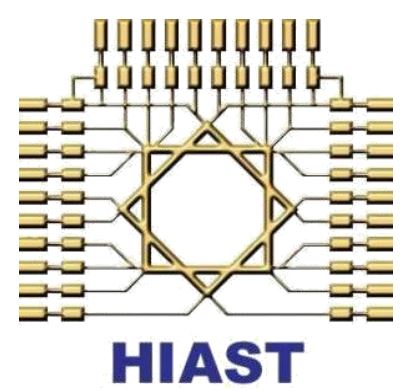
\includegraphics[width=0.9\linewidth]{hiast}
\end{wrapfigure}

\ \\[\lineSeparationLength]
Syrian Arab Republic \\[\lineSeparationLength]
Higher Institute for Applied Sciences and Technology \\[\lineSeparationLength]
Informatics Department \\[\lineSeparationLength]
Fourth Year
}

\vspace{25mm}
{\let\newpage\relax\maketitle}

\vspace{-10mm}
\begin{center}
Keywords: minimum vertex cover, NP-complete, genetic algorithms,\\
combinatorial optimization, approximation algorithms.
\end{center}

\vspace{5mm}
\begin{center}
\begin{onehalfspacing}

\begin{tabular}{r l}
Author:					&	\textit{Farouk Hjabo} \\
Academic Supervisor:	&	\textit{Dr. Said Desouki} \\
General Supervisor:		&	\textit{Dr. Kadan Aljoumaa} \\
Langauge Supervisor:	&	\textit{Mr. Fahmi Alammareen} \\
\end{tabular}

\end{onehalfspacing}
\end{center}

\vfill
\centerline{\date{\today}}
\thispagestyle{empty}
\pagebreak

% abstract page
\phantomsection\addcontentsline{toc}{section}{Abstract}

\begin{abstract}
Remarkable results obtained from the application of a
genetic algorithm to the minimum vertex cover problem
are reported, and tested against the results of the
best known heuristic algorithm for graphs of sizes 100 and 200 nodes.
In contrast to many other approximation algorithms that use problem-specific
knowledge, the approach presented relies on a graded penalty term component
of the fitness function to penalize infeasible solutions.
\end{abstract}

\vfill

\noindent
\textit{
``It is not the strongest of the species that survives,
nor the most intelligent, but the one most responsive
to change.''
}
\begin{flushright}
\setlength{\parskip}{0em}
--- Charles Darwin
\end{flushright}

\pagebreak


% table of contents page
\setstretch{0.5}
\phantomsection\addcontentsline{toc}{section}{Contents}
\tableofcontents
\setstretch{1.0}


\pagebreak

% List of Figures and Tables
\phantomsection\addcontentsline{toc}{subsection}{List of Figures}
\listoffigures

\phantomsection\addcontentsline{toc}{subsection}{List of Tables}
\listoftables

\phantomsection\addcontentsline{toc}{subsection}{Abbreviations}
\section*{Abbreviations}  % Set the left side page header to "Abbreviations"
\begin{onehalfspacing}
\begin{tabular}{l l}

\indent
GA		&	\textbf{G}enetic \textbf{A}lgorithm \\

\indent
mvc		&	\textbf{M}inimum \textbf{V}ertex \textbf{C}over \\

\indent
mvcp	&	\textbf{M}inimum \textbf{V}ertex \textbf{C}over \textbf{P}roblem \\

\end{tabular}
\end{onehalfspacing}

\pagebreak


% first page starts here
\pagenumbering{arabic}

\section{Introduction}
\label{sec:intro}
Once the NP-hardness of a combinatorial optimization
problem is established, the search for an optimal solution
is abandoned.
Our goal then becomes one of finding good heuristics
for that problem.
That is, we try to find approximation algorithms
that have polynomial time complexities and return near-optimal
solutions.
In most cases, the heuristic is problem dependent; it is tailored to specific problem
it is trying to solve, and it is tightly coupled with observations made about the problem.
The \textit{minimum vertex cover} problem is a typical example of such
problems \cite{wolfram:mvc}.
Due to its numerous applications especially in various
matching problems, the problem is not abandoned and it has many
approximation algorithms.

In this work, we present an alternative approach that
uses \textit{genetic algorithms} as a generalized heuristic for
solving NP-hard combinatorial optimization problems.
These algorithms have been successfully applied to a broad
range of problems.
This wide range can be tackled by genetic algorithms
mainly due to the fact that these algorithms work with an
encoding of the problem rather than the characteristics
of that problem.
Remarkable results were obtained and compared to the results of the
best known heuristic algorithm for the mvcp.

The outline of this paper is as follows: Firstly, Section~\ref{sec:ga} gives a
short introduction to genetic algorithms, and explains briefly how they work.
Section~\ref{sec:mvcp} introduces the mvcp with two of its main heuristics,
and explains its representation for an application of the genetic algorithm.
Lastly, Section~\ref{sec:exper} presents our experimental results and
points out the notable observations that can be drawn from these results.



\section{Genetic Algorithms}
\label{sec:ga}
\subsection{The Intuition Behind GAs}
Genetic Algorithms (GAs) \cite{coley, goldberg} are population based
search algorithms, where by repeated use of genetic operations,
such as \textem{mutation}, \textem{selection}, \textem{crossover}, etc...
Successive new generations of better populations in the direction of
search objectives are created.
They are inspired by Darwinian principles
based on natural evolution.
In other words, the main idea behind genetic
algorithms is that only the \textem{fittest} individuals will survive
among generations of evolution.

Main advantage of genetic algorithms is that they ideally do not make
any assumption about the underlying problem, hence they are suitable to tackle
a wide range of diverse problems in
engineering, art, biology, economics, marketing, genetics,
operations research, robotics, social sciences, physics, politics, chemistry,
etc... \cite[ch.~6]{coley}

\noindent
So what is a GA? A typical GA consists of the following~\cite[ch.~1]{coley}:
\vspace{-5mm}
\begin{enumerate}
\setlength{\parskip}{0em}

\item
a number, or \textem{population}, of candidate solutions to the problem.

\item
a way of calculating how good or bad the individual solutions within the
population are.
i.e. how \textem{fit} an individual is?

\item
a method for mixing fragments of the better solutions to form new, on
average even better solutions.
Which permits the population to \textem{evolve} naturally.

\end{enumerate}

\subsection{Typical GA Schema}
The basic iteration cycle of a genetic algorithm proceeds on a population
of individuals, each of which represents a search point in the space
of potential solutions of a given optimization problem.
In case of a canonical genetic algorithm, each individual is a binary vector
$ \vec{x} = ( x_1, \dots, x_n ) \in \{0, 1\}^n $
of fixed length $n$.
The fitness function
$ f: \{0, 1\}^n \rightarrow \mathbb{R} $
provides a quality measure which is used by the selection procedure to direct
the search towards regions of the search space where the
average fitness of the population increases.
The recombination operator
allows for the exchange of information between different individuals,
and mutation introduces innovation into the population.
This cycle is repeated until a termination criterion is fulfilled.
In most cases, the algorithm is terminated after a certain number of
iterations of the basic cycle or when a satisfactory fitness
level has been reached.\\
Refer to figure~\ref{fig:ga} for a visual representation of this process,
and refer to algorithm~\ref{alg:ga} for a more concise description.

\begin{figure}[!htb]
\centering
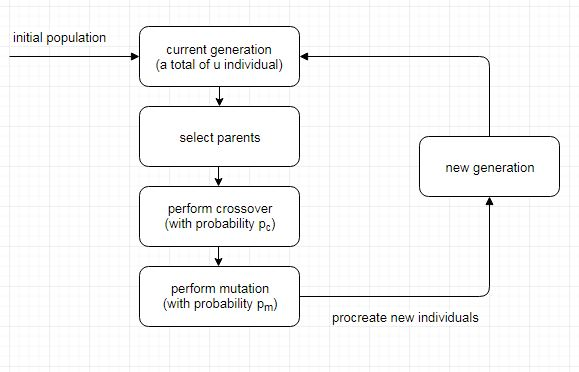
\includegraphics[width=1\textwidth]{ga}
\caption{General schema for genetic algorithms}
\label{fig:ga}
\end{figure}

\paragraph{Initialization}
The population size (denoted as $u$) depends on the nature of the problem,
but typically contains several hundreds or thousands of possible solutions.
Often, the initial population is generated randomly, allowing the entire range
of possible solutions (the search space).
Occasionally, the solutions may be `seeded' in areas where optimal solutions
are likely to be found.

\paragraph{Selection}
Normally, selection in genetic algorithms is a probabilistic operator
which uses the relative fitness
$ p_s \left( \vec{x_i} \right) = 
f \left( \vec{x_i} \right) / \sum_{j=1}^uf \left( \vec{x_j} \right) $
to serve as selection probabilities ($u$ denotes the population size).
This selection operator is called proportional selection.
It is commonly used; as intuitively the more fit a solution is the more we
want it to affect the next generations.\\
If the problem under consideration is a minimization one,
or if the fitness function can take negative values,
then $ f \left( \vec{x_i} \right) $ has to be
linearly transformed before calculating selection probabilities.
This technique known as linear dynamic scaling is commonly used
in genetic algorithms \cite[pp.~123--124]{goldberg}.

\paragraph{Crossover}
The recombination (crossover) operator allows for the
exchange of information between different individuals.
The original one-point crossover \cite{holland} works on two parent individuals
by choosing a crossover point $ \chi \in \{1, \dots, n-1 \} $
at random and exchanging all bits after the $ \chi^{\text{th}} $ one
between both individuals.
Therefore, two new off-springs will be formed.\\
For example, if the two parents were encoded as $(111, 000)$ and we chose $\chi = 2$
then the new two off-springs will be $(110, 001)$.
The crossover rate $ p_c \ (\text{e.g. } p_c \approx 0.6) $
determines the probability to undergo crossover (see algorithm~\ref{alg:ga} line~\ref{alg:crossover}),
this allows the two parents to be present in the next generation; as crossover is not mandatory.
Moreover, the value of $p_c$ indicates the ratio of new off-springs in the next generation.\\
The crossover operator can be extended to a generalized
multi-point crossover or even to uniform crossover,
where it is randomly decided for each bit
whether to exchange it or not.
The strong mixing effect introduced by uniform crossover
is sometimes helpful to overcome local optima.

\paragraph{Mutation}
Innovation (new information) is introduced into the
population by means of mutation, which works by inverting
bits with a small probability $p_m \ (\text{e.g. } p_m \approx 0.001)$
(see algorithm~\ref{alg:ga} lines~\ref{alg:m1}~\ref{alg:m2} for clarity).
Though mutation is often interpreted as a rather unimportant operator
in genetic algorithms \cite{holland}, recent theoretical
work gives strong evidence for an appropriate choice of a
mutation rate $ p_m = 1/n $ on many problems \cite{2:misp, 12:misp}.

\begin{algorithm}[!htb]
\caption{GenticAlgorithm$\left( n, u, p_c, p_m, f \right)$}
\label{alg:ga}

\begin{algorithmic}[1]


\State $ P \gets \{ \} $
\Comment{$P$ contains the population}
\Loop \ $u$ times
\Comment{initialization}
\State add a randomly generated binary vector of length $n$ to $P$
\EndLoop

\While{termination criterion is not fulfilled}
\State $Q \gets \{ \}$
\Comment{$Q$ will hold the new generation}
\Loop \ $u/2$ times

\State select $x, y$ from $P$ using proportional selection
\Comment{selection}
\State with probability $p_c$ perform crossover between $x, y$
\Comment{crossover}
\label{alg:crossover}
\State for each bit in $x$ flip it with probability $p_m$
\Comment{mutation}
\label{alg:m1}
\State for each bit in $y$ flip it with probability $p_m$
\Comment{mutation}
\label{alg:m2}
\State add $x, y$ to $Q$

\EndLoop

\State $P \gets Q$
\EndWhile


\end{algorithmic}

\end{algorithm}



\section{The Minimum Vertex Cover Problem}
\label{sec:mvcp}
The problem of finding a minimum vertex cover is a classical
optimization problem in computer science and is a typical
example of an NP-complete optimization problem \cite{wolfram:mvc}
that has approximation algorithms.
The mvcp of an undirected graph $G = (V, E)$ where $V$ is
the set of vertices and $E$ denotes the set of edges,
consists in finding the smallest subset $V' \subseteq V$ such that
$\forall \langle i, j \rangle \in E$, we have $i \in V'$ or $j \in V'$ (or both).
$V'$ is said to be a vertex cover of $G$.

The following is a formal definition of
the mvcp in which we make use of Stinson's terminology
for combinatorial optimization problems~\cite{14:mvcp}:

{
\setlength{\parskip}{0em}
\paragraph{Problem instance:}
A graph $G = (V, E)$, where $V = \{1, 2, \dots, n\}$
is the set of vertices and $E \subseteq V \times V$ the
set of edges.
An edge between vertices $i, j$ is denoted
by the pair $\langle i, j \rangle \in E$.
We define the adjacency matrix $e_{ij}$ according to:
\[
e_{ij} =
\begin{cases}
1 & \text{if } \langle i, j \rangle \in E \\
0 & \text{otherwise}
\end{cases}
\]
On particular, we have $e_{ii} = 0$.

\paragraph{Feasible solution:} A set $V' \subseteq V$ such that
$\forall \langle i, j \rangle \in E, i \in V' \vee j \in V'$
\paragraph{Objective function:} The size $|V'|$ of the vertex cover $V'$.
\paragraph{Optimal solution:} a vertex cover $V'$ that minimizes $|V'|$.
}

An interesting property of the mvcp is that by
solving it, we also have a solution for two other
graph problems: the \textit{maximum independent set problem}
(given $G = (V, E)$, find the largest subset $V' \subseteq V$
such that $\forall i, j \in V', \langle i, j \rangle \notin E$)
and the \textit{maximum clique problem}
(given $G = (V, E)$, find the largest subset $V' \subseteq V$
such that $\forall i, j \in V', \langle i, j \rangle \in E$)
The close relationship between these problems is characterized
by the following lemma \cite{6:misp}.
\begin{lemma}
\label{lem}
\ \\[3mm]
For any graph $G = (V, E)$ and $V' \subseteq V$, the following
statements are equivalent:
\begin{itemize}
\vspace{-3mm}
\setlength{\parskip}{0.5em}
\item $V'$ is the minimum vertex cover of $G$.
\item $V - V'$ is the maximum independent set in $G$.
\item $V - V'$ is the maximum clique in $\bar{G} = (V, \bar{E})$,\\[1mm]
where
$\bar{E}=\left\{ \langle i, j \rangle\in V \times V :
\langle i, j \rangle \notin E \right\}$
\end{itemize}
\end{lemma}

Consequently, one can obtain a solution of the maximum independent set
problem by taking the complement of the solution to the minimum vertex cover
problem. A solution to the maximum clique problem is obtained by
taking the complement of the minimum vertex cover of $\bar{G}$.

\subsection{Related Algorithms}
\label{sec:ra}
Since we are interested in covering all the edges of the
given graph by using as few nodes as possible, one might
be tempted to use a greedy-based heuristic to tackle the
mvcp.
The algorithm consists in repeatedly selecting a
vertex of highest degree (the node that covers as many
of the remaining edges as possible), and removing all
of its incident edges.
This is not a good strategy as was demonstrated
by Papadimitriou and Steiglitz \cite[p.~407]{10:mvcp}.

They considered regular graphs\footnote{%
by ``regular graphs'' we don't refer to the definition where
each vertex has the same degree.
}, each of which consists of three levels.
The first two levels have the same
number of nodes while the third level has two nodes less
than the number of nodes found on the previous two
levels.
More precisely, each graph consists of $n = 3k + 4 \ (k \geq 1)$
nodes; $k+2$ nodes on the first level, labeled $1, 2, \dots, k+2$;
followed by $k+2$ nodes on the second level, labeled $k+3, \dots, 2k+4$;
while the $k$ nodes of the third level are labeled $2k+5, \dots, 3k+4$.
The regular graph for $k = 3$ can be found in figure~\ref{fig:ps}.
A minimum vertex cover is obtained by choosing all
the nodes of the second level, but the greedy strategy
would start with the nodes of the third level, since these
have highest degree. Consequently, the greedy strategy
finds a solution of size $2k + 2$ (since it has to select $k + 2$
nodes in addition to the nodes of the third level), while
the optimal solution has size $k + 2$.

However this algorithm is not totally useless. It may be shown that it always
achieves the ratio $\Theta(\lg n)$\footnote{$f(n) = \Theta(g(n)) \iff
\exists \alpha, \beta, n_0 : \forall n \geq n_0, \ 
\alpha \cdot g(n) \leq f(n) \leq \beta \cdot g(n)$ \cite[pp.~41--43]{cormen}},
where $n$ is the number of vertices.
That is, if $C^*(n)$ is the size of the optimal
solution and $C(n)$ is the size of the solution found by the greedy
algorithm. Then we have $\frac{C(n)}{C^*(n)} = \Theta(\lg n)$ \cite[p.~323]{9:mvcp}.

\begin{figure}[!htb]
\centering
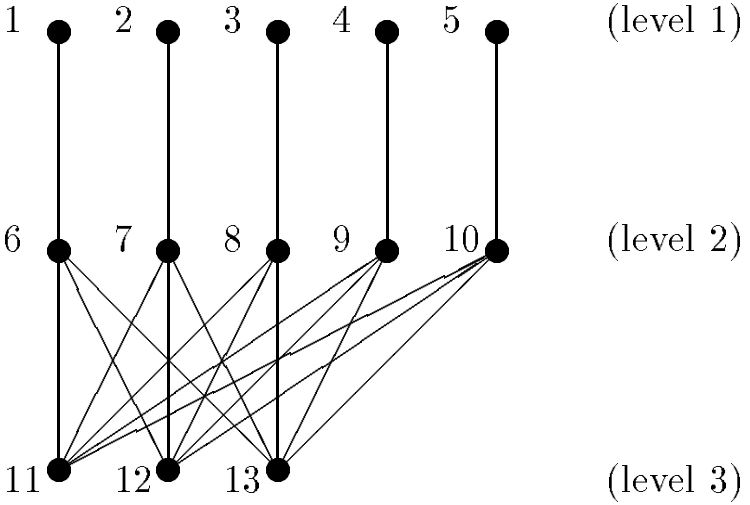
\includegraphics[width=0.5\textwidth]{ps}
\caption[The regular graph after Papadimitriou
and Steiglitz for $k=3$]
{Construction of the regular graph after Papadimitriou
and Steiglitz with $k=3$}
\label{fig:ps}
\end{figure}

Fortunately, a simpler and better algorithm exists.
The following simple algorithm is surprisingly the
best approximation algorithm known for the mvcp \cite[p.~301]{9:mvcp}.

\begin{algorithm}[!htb]
\caption{vercov($G = (V, E)$)}
\label{alg:vercov}
\begin{algorithmic}[1]

\State $C \gets \{ \}$
\Comment{$C$ contains the vertex cover being constructed}
\State $E' \gets E$
\While{$E' \neq \phi$}
\State randomly choose $ \langle u, v \rangle \in E'$
\label{alg:rand}
\State $C \gets C \cup \{u, v\}$
\State $E' \gets E' -
\{ \langle x, y \rangle \in E' : x=u \vee y=v \vee x=v \vee y=u \}$
\State \Comment{remove from $E'$ every edge incident on either $u$ or $v$}
\EndWhile
\State \Return $C$

\end{algorithmic}
\end{algorithm}

This is a \textit{2-approximation algorithm}. Which means that
the size of the vertex cover
it returns is guaranteed to be no more than twice the
size of an optimal vertex cover \cite[p.~968]{cormen}.
More precisely, if $C^*$ is the size of the optimal
solution and $C$ is the size of the solution returned by algorithm~\ref{alg:vercov}
then the inequality $C \leq 2C^*$ must hold (notice that here the approximation
doesn't depend on the number of vertices).

\subsection{GA for the mvcp}
\label{sec:GAmvcp}
In order to apply genetic algorithm to solve the mvcp, a cover $V'$ is represented
by a binary vector $\vec{x} = x_1x_2 \dots x_n$ where $x_i = 1$ if
the $i^{\text{th}}$ node is in $V'$, and $x_i = 0$ if it is not.
Using this representation, genetic algorithm is applied to minimize the following
fitness function~\cite{mvcp-back}:
\begin{equation}
\label{eq:f}
\begin{split}
f(\vec{x})	&= \sum_{i=1}^{n} \left( x_i+n \cdot (1-x_i) \cdot
			   \sum_{j=i}^{n} (1-x_j) e_{ij} \right) \\
 			&= \sum_{i=1}^{n} x_i + n \cdot \sum_{i=1}^{n}
			   \sum_{j=i}^{n} (1-x_i) \cdot (1-x_j) \cdot e_{ij}
\end{split}
\end{equation}

The term $ \sum_{i=1}^{n} x_i $ of $ f(\vec{x}) $ determines the size of the
potential vertex cover represented by $\vec{x}$, while the term
$ n \cdot \sum_{i=1}^{n} \sum_{j=i}^{n} (1-x_i) \cdot (1-x_j) \cdot e_{ij} $
penalizes sets $V'$ that
are not covers by adding a penalty of magnitude $n$ for
each edge $e_{ij}$ for which $i \notin V' \wedge j \notin V'$
(note that $e_{ii}$ is previously defined to be zero).
Consequently, any infeasible solution will have a fitness greater than
or equal to $n$. And for any feasible solution the second term will
drop to zero, making the fitness value of the worst feasible solution at most $n$.

This fitness function was developed according to the
following design principles that are important for a
successful penalty function approach \cite{7:mvcp, 11:mvcp}:
\begin{itemize}
\vspace{-4mm}

\item Infeasible binary vectors are guaranteed to yield fitness
values which are inferior to fitness values of
the worst feasible solutions.

\item The penalty should be graded, i.e., fitness values
should improve as solutions approach feasible regions
of the search space. In other words, the more edges a solution
covers, the fitter it is. notice that this is guaranteed by the
second term in equation~\ref{eq:f}, where for each uncovered edge
the fitness is penalized with the value of $n$.
\end{itemize}

The experiments reported in section~\ref{sec:er} are performed
by using a genetic algorithm with a population size of
$u = 50$, mutation rate $p_m = 1/n$, crossover rate
$p_c = 0.6$, proportional selection, and two-point crossover \cite{mvcp-back}.
As reported in \cite{2:mvcp, 12:mvcp}, the latter is expected to perform
better than the traditional one-point crossover.
A bound for the total number
of fitness function evaluations is set as the termination
criterion \cite{mvcp-back}, see section~\ref{sec:er} for details.


\section{Experiments}
\label{sec:exper}
For the experimental tests,
the genetic algorithm software package GENEsYs is used \cite{1:misp}.
This implementation is based on the widely used GENESIS software by Grefenstette \cite{5:mvcp},
but allows for more  flexibility concerning genetic operators and data monitoring.
The parameter settings for the experiments are
given in section~\ref{sec:GAmvcp}.


\subsection{Experimental Results}
\label{sec:er}

\paragraph{Test set~1:}
Multiple problem instances are used to demonstrate the applicability of GAs to tackle the mvcp.
The results in table~\ref{tbl:t1}
and table~\ref{tbl:t2} correspond to the test set~1, which consists of
five random graphs of size $n = 100$ with different
edge densities $d$.
Densities $d \in \{0.1, 0.2, 0.3, 0.4, 0.5\}$ are used respectively.
An edge density of $d = 0.1$ means that an edge is placed between two
nodes with a probability of 0.1.
Moreover, we construct the graphs in a way that guarantees an optimum of quality 55 \cite{mvcp-back}.
i.e. we use algorithm~\ref{alg:gen} with $k = 55$ to generate random graphs.\\
In addition, the regular graphs introduced by
Papadimitriou and Steiglitz and described in section~\ref{sec:ra} are used.
Recall that these graphs contain $n=3k+4 \ (k \geq 1)$ nodes distributed on three levels.
They can be scaled up by choosing high values for $k$.
A graph instance of the regular graph of size $n = 100 \  (k=32)$ is chosen.

\begin{algorithm}[!htb]
\caption{GenerateRandomGraph$(n, d, k)$}
\label{alg:gen}
\begin{algorithmic}[1]
\algnotext{EndFor}
\algnotext{EndIf}


\State randomly select $V' = \{i_1, \dots, i_k\} \subseteq V = \{1, \dots, n\}$
\State
\Comment{randomly select k different nodes, these nodes will hold a potential mvc}
\For{$i$}{$1$}{$n-1$}
\For{$j$}{$i+1$}{$n$}
\If{$(\text{Random(0, 1)} \leq d) \wedge (i \in V' \vee j \in V')$}
\State $e_{ij} = 1$
\Else
\State $e_{ij} = 0$
\EndIf
\EndFor
\EndFor


\end{algorithmic}
\end{algorithm}

\paragraph{Termination:}
As a termination criterion for the genetic algorithm,
a bound for the total number of fitness function evaluations is set.
For example The total number of function evaluations per single run
is chosen to be $2 \cdot 10^4$ in table~\ref{tbl:t1}.
That is, the algorithm terminates when $2 \cdot 10^4$ evaluations of the fitness function
had occurred.
This bound is indicated as an index $t$ in the notation $f_t(\vec{x})$.
Consequently, only a small fraction of the search space is explored by the genetic algorithm.
This fraction is about
$ 2 \cdot 10^4 / 2^{100} \approx 1.6 \cdot 10^{-24} \% $
for test set~1.
And it is about $ 4 \cdot 10^4 / 2^{200} \approx 2.5 \cdot 10^{-54} \% $ for test set~2.

\paragraph{Table~\ref{tbl:t1}:}
For each graph in test set~1, a total of
$N = 100$ independent runs of the genetic algorithm is performed.
The results are summarized in table~\ref{tbl:t1} for the best
fitness values that were encountered during the 100 runs.
For each problem instance, the different fitness values that were
obtained and their frequencies are recorded.
Furthermore, the average fitness value $\bar{f}$ over
all 100 runs is indicated at the bottom of the table.\\
For example, the first column in table~\ref{tbl:t1} indicates
that the best obtained fitness value in 1 of the 100 runs was $f(\vec{x}) = 53$,
the best obtained fitness value in 1 of the 100 runs was $f(\vec{x}) = 54$,
the best obtained fitness value in 3 of the 100 runs was $f(\vec{x}) = 55$, and so on...
And the average of these values is indicated by $\bar{f}$, which is the average value of
the best obtained fitness values over the 100 runs.


\begin{table}[!htb]
\centering
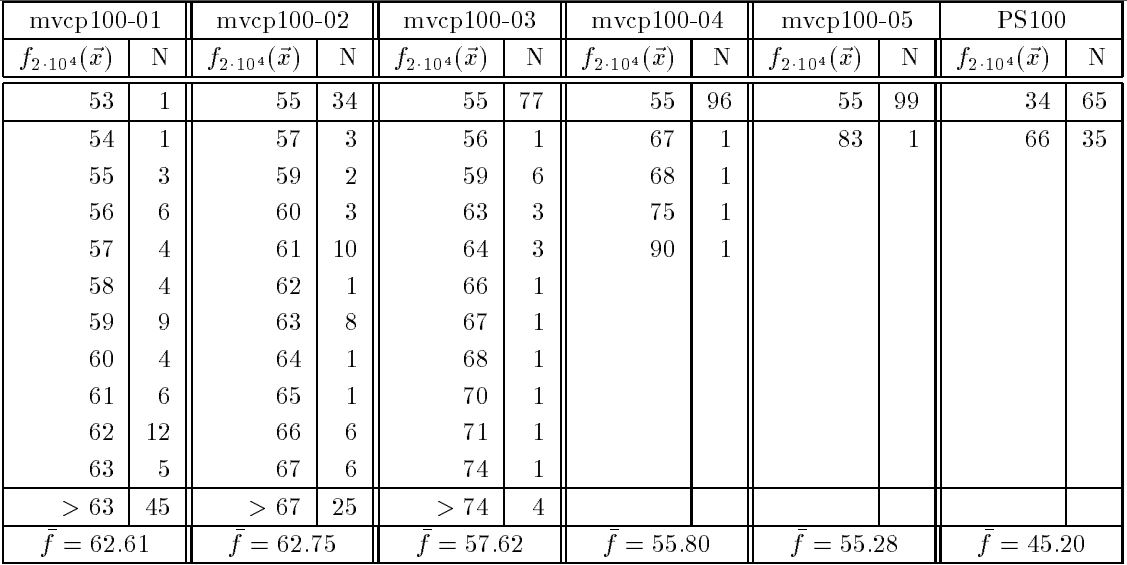
\includegraphics[width=1\textwidth]{t1}
\caption[Results obtained by GA for graphs in test set~1]{%
Experimental results obtained by the genetic algorithm for five random graphs of size $n = 100$ with edge density: $d = 0.1$ (``mvcp100-01''), $d = 0.2$ (``mvcp100-02''), $d = 0.3$ (``mvcp100-03''), $d = 0.5$ (``mvcp100-04''), $d = 0.5$ (``mvcp100-05'') and the regular graph of size $n = 100 \ (k=32)$ from Papadimitriou and Steiglitz (``PS100'').%
}
\label{tbl:t1}
\end{table}

\paragraph{Table~\ref{tbl:t2}:}
For each of the problems in the test set~1, a total of $N=100$
independent runs of the vercov heuristic is performed.
The results are summarized in table~\ref{tbl:t2}.
Notice that for one problem instance, the results may differ in each run due to the
non-determinism of the algorithm (see algorithm~\ref{alg:vercov} line~\ref{alg:rand}).

\begin{table}[!htb]
\centering
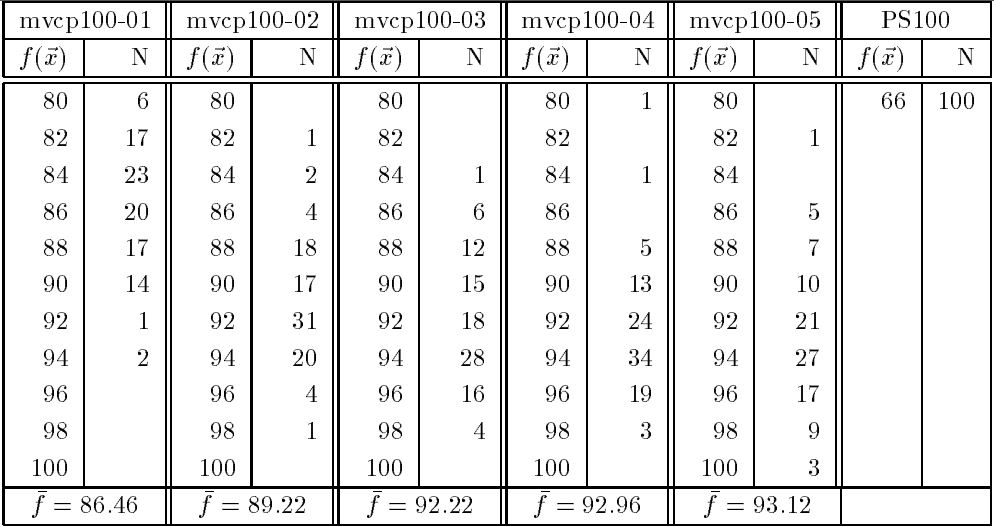
\includegraphics[width=1\textwidth]{t2}
\caption[Results obtained by vercov heuristic for graphs in test set~1]{%
Experimental results obtained by the vercov heuristic for five random graphs of size $n = 100$ with edge density: $d = 0.1$ (``mvcp100-01''), $d = 0.2$ (``mvcp100-02''), $d = 0.3$ (``mvcp100-03''), $d = 0.5$ (``mvcp100-04''), $d = 0.5$ (``mvcp100-05'') and the regular graph of size $n = 100 \ (k=32)$ from Papadimitriou and Steiglitz (``PS100'').%
}
\label{tbl:t2}
\end{table}

\paragraph{Test set~2:}
To test the behaviour of the genetic algorithm
as well as the vercov heuristic for an even
larger problem size, The same experiments
were performed for larger graphs.
The results in table~\ref{tbl:t3}
and table~\ref{tbl:t4} correspond to test set~2,
which consists of five random graphs of size
$n = 200$ with different edge densities $d$.
Densities $d \in \{0.1, 0.2, 0.3, 0.4, 0.5\}$ are used.
Moreover, we construct the graphs in a way that guarantees an optimum of quality 110
(see algorithm~\ref{alg:gen}, we set $k = 110$).
In addition to a graph instance of the regular graphs introduced by
Papadimitriou and Steiglitzof of size $n = 220 \ (k=66)$.
In this case, the genetic algorithm
was allowed to run for $4 \cdot 10^4$ function evaluations.\\
The corresponding results obtained by the
genetic algorithm are shown in table~\ref{tbl:t3}, while the results
from the vercov heuristic are shown in table~\ref{tbl:t4}.
See the previous paragraphs for a better understanding of these results.

\begin{table}[!htb]
\centering
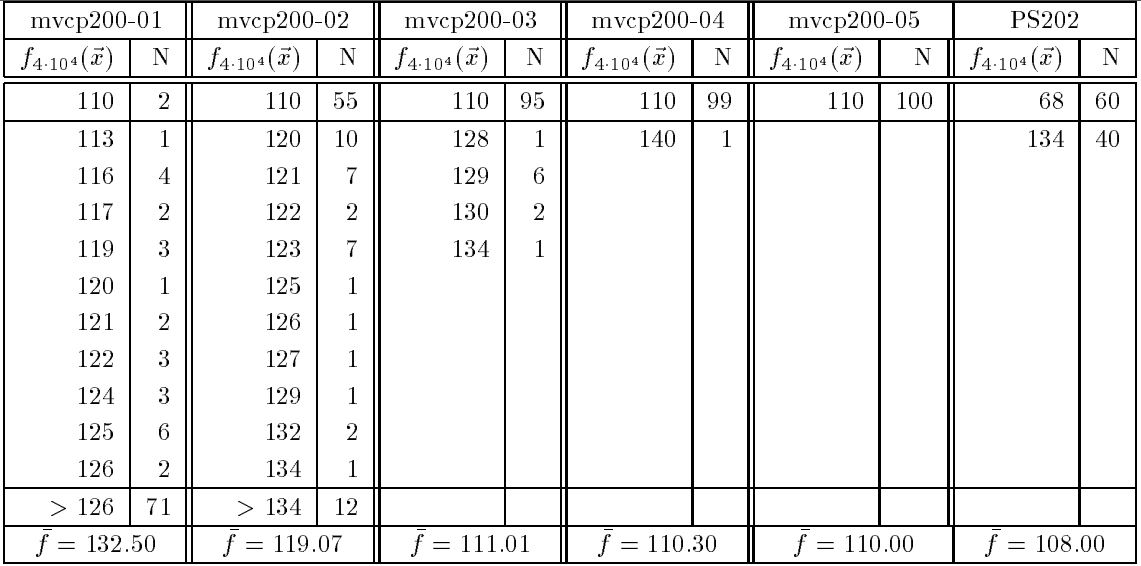
\includegraphics[width=1\textwidth]{t3}
\caption[Results obtained by GA for graphs in test set~2]{%
Experimental results obtained by the genetic algorithm for five random graphs of size $n = 200$ with edge density: $d = 0.1$ (``mvcp200-01''), $d = 0.2$ (``mvcp200-02''), $d = 0.3$ (``mvcp200-03''), $d = 0.5$ (``mvcp200-04''), $d = 0.5$ (``mvcp200-05'') and the regular graph of size $n = 202 \ (k=66)$ from Papadimitriou and Steiglitz (``PS202'').%
}
\label{tbl:t3}
\end{table}

\begin{table}[!htb]
\centering
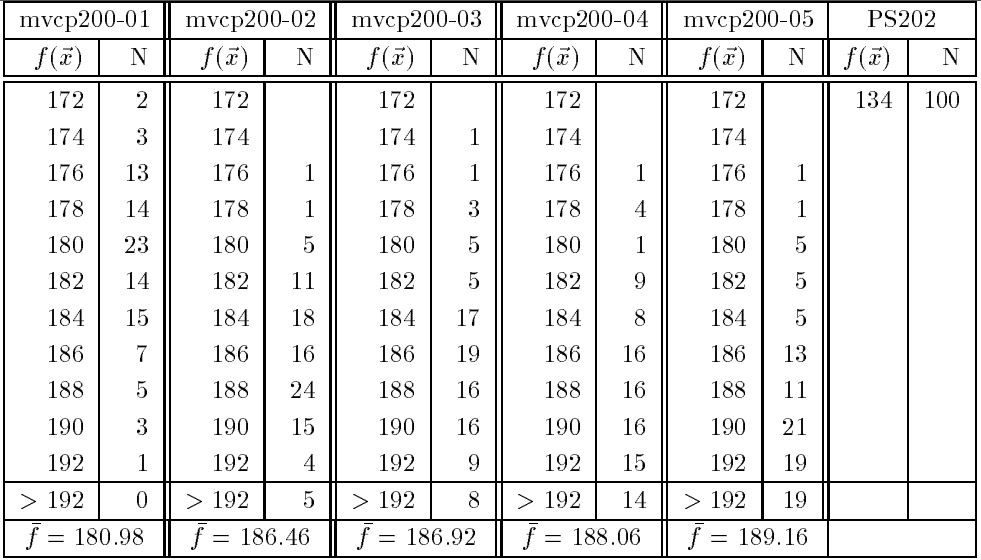
\includegraphics[width=1\textwidth]{t4}
\caption[Results obtained by vercov heuristic for graphs in test set~2]{%
Experimental results obtained by the vercov heuristic for five random graphs of size $n = 200$ with edge density: $d = 0.1$ (``mvcp200-01''), $d = 0.2$ (``mvcp200-02''), $d = 0.3$ (``mvcp200-03''), $d = 0.5$ (``mvcp200-04''), $d = 0.5$ (``mvcp200-05'') and the regular graph of size $n = 202 \ (k=66)$ from Papadimitriou and Steiglitz (``PS202'').%
}
\label{tbl:t4}
\end{table}


\subsection{Experimental Conclusions}
From these tables, a number of interesting conclusions
can be drawn.
For the random graphs used to compare the
genetic algorithm and the vercov heuristic,
it is known by construction that an optimum of
quality 55 exists for test set~1,
(respectively, an optimum of quality 110 exists
for the test set~2).
This optimum is likely to be the global optimum.
And it is found by the genetic algorithm at least once
within the $N = 100$ runs that were performed.

Moreover, the randomly constructed problems quickly
become simpler for the genetic algorithm when the edge
density is increased.
For an edge density of $d \in \{0.4, 0.5\}$, the
genetic algorithm almost surely finds the global optimum
of the problems, while vercov heuristic gives
a relatively terrible results.

In case of the regular graph after Papadimitriou and
Steiglitz, the genetic algorithm is able to find the global
optimum in about $2/3$ of all runs, while the remaining
runs identify a solution of quality $2k + 2$.
Whereas, vercov heuristic gives a solution of
quality $2k + 2$ in all of the 100 runs as expected \cite{10:mvcp}.
Recall that the graphs are constructed
so as to force the vercov heuristic into yielding solutions
of quality $2k + 2$.
The random choice of edges (line~\ref{alg:rand} of algorithm~\ref{alg:vercov})
implies that nodes from either layers one and two, or layers two and three
are involved in the solution being constructed,
which in turn implies that two layers have to be part of the solution
found by the algorithm.

For the randomly constructed graphs, the vercov heuristic
performs poorly.
It barely finds solutions of quality 80 (for graphs of size 100)
and 172 (for graphs of size 200).
Moreover, notice that the quality of its solutions are dominated
by the quality of the solutions found by the genetic algorithm;
the worst solutions found by the genetic algorithm are almost as
good as the best solutions found by the vercov heuristic.

The average performance of the vercov heuristic (surprisingly)
decreases as the edge density is increased;
i.e. the problems become even harder for the vercov heuristic
while they become much simpler for the genetic algorithm when
the edge density increases.
The average fitness found by the genetic algorithm is notably
better than the one found by the vercov heuristic.
One can demonstrate this by calculating
the ratio of the absolute (or equivalently, the relative) error.
For example, for the first problem instance,
let $\bar{f}_1, \bar{f}_2$ be the average found by
the genetic algorithm, vercov heuristic respectively.
We have $ (\bar{f}_2 - 55) / (\bar{f}_1 - 55) = (86.46 - 55)/(62.61 - 55) \approx 4 = 400\%$
that is, the error was reduced by a factor of 4.


\section{Conclusion}
\label{sec:conc}
This work has demonstrated that genetic algorithms can
be used in a fairly straightforward way to find good
approximative solutions for NP-hard problems, namely
the minimum vertex cover problem.
The robustness of the presented solution along with
the positive results obtained support the idea
that genetic algorithms are a desirable approach for tackling
these type of problems.
To tackle a new problem, rather than having to construct
tailored heuristics to handle the problem under consideration,
we advocate the use of genetic algorithms where the
only change to perform is the formulation of a new fitness
function.

%\pagebreak


\phantomsection\addcontentsline{toc}{section}{References}
%\bibliographystyle{abbrv}
%\bibliography{references}
\printbibliography

% end of document
\end{document}

